%##############################################
\chapter{The top quark}
%##############################################
\label{ch:top}

\intro{The theoretical background of the top quark and its production mechanisms are introduced in this chapter. A feature of the top quark is that its spin orientation is preserved in decays which allows to study the coupling structure in various processes. In particular, the production of single top quarks in $t$~channel via W~boson exchange is detailed which is the main subject of the measurements within this thesis. Furthermore, \gls{bsm} production mechanisms, detectable through an alteration of the Wtb coupling structure, are discussed as well using an effective approach. The chapter is concluded with a discussion of recent experimental results.}


The top quark is the heaviest known fundamental particle so far. Its high mass of $m_\mathrm{t}=172.44\pm0.49~\GeV$~\cite{Khachatryan:2015hba} is close to the minimum of the Higgs potential. This implies a Yukawa coupling of $|\lambda_\mathrm{t}|\approx 1$. All other Yukawa couplings are however of the order of $10^{-2}$ instead. The top quark may therefore play an important role in understanding the mechanisms of electroweak symmetry breaking itself. Furthermore, top quarks are excellent probes to search for \gls{bsm} physics. For example, many extensions of the \gls{sm} predict additional $\mathrm{W}^{\prime}$ and $\mathrm{Z}^{\prime}$ bosons which are heavier versions of their \gls{sm} counterparts and can decay into top quarks. Other \gls{bsm} models can have an extended Higgs sector including additional neutral and charged Higgs bosons which may couple to top quarks predominantly due to its high mass~(see Ref.~\cite{Boos:2006xe} and references therein).

Historically, the top quark was discovered in 1995 by the \gls{cdf}~\cite{Abe:1995hr} and \gls{d0}~\cite{Abachi:1994td} collaborations at the Tevatron collider at Fermilab using proton-antiproton collision data. They observed the production of top quark-antiquark pairs which occurs through strong interactions. Already before the direct observation of this process an attempt to explain CP-violation by introducing the \gls{ckm} matrix and hence postulating a third quark generation~\cite{Kobayashi01021973} which was followed by the discovery of the bottom quark~\cite{Augustin:1975yq,PhysRevLett.39.252} hinted strongly towards the top quark's existence. Another milestone was the observation of single top quark production which occurs through electroweak interactions only. This process was discovered in 2009 at the Tevatron collider as well~\cite{PhysRevLett.103.092002,PhysRevLett.103.092001}. The lower cross section together with the overwhelming background necessitated the use of sophisticated analysis techniques such as multivariate classifiers and the matrix element method~\cite{Mitrevski}.

With the start of the physics program at the \gls{lhc} in 2009, the production mechanisms of top quarks can be probed with unprecedented precision. This thesis focuses on the electroweak production of single top quarks at center-of-mass energies of $8~\TeV$ and $13~\TeV$.


%##############################################
\section{Decay and W~boson polarization}
%##############################################
\label{sec:theory-top-quark-decay}

The top quark decays into a W boson and a b quark almost exclusively due to the \gls{ckm} matrix element $\vtb$ which is found experimentally to be $\vtb\gg\vts,\vtd$ and close to 1. The W boson can be on-shell since $m_\mathrm{W}<m_\mathrm{top}$ which favors this decay channel via electroweak interactions and leads to a very short lifetime of only $1/\Gamma_\mathrm{t}\approx 5\cdot10^{-25}~\mathrm{s}$~\cite{Olive:2016xmw}. This does not allow the formation of bound states involving top quarks~\cite{BIGI1986157}. Furthermore, the lifetime is even shorter than the typical hadronization timescale of $1/\Lambda_\mathrm{QCD}\approx 10^{-23}~\mathrm{s}$. Hence, soft gluons cannot radiate from the top quark before it decays which keeps its spin coherent. The top quark spin orientation can be inferred from the angular distributions of its decay products since electroweak interactions via $\mathrm{W}$ boson exchange feature a \gls{va} coupling structure. This offers the possibility to study the polarization of top quarks from angular distributions in various processes. For such studies, a spin axis has to be chosen along which the top quark spin is quantized.

Independent of the production process, the polarization states of the $\mathrm{W}$~boson can be investigated in the leptonic top quark decay chain $\mathrm{t}\to\mathrm{b}\ell\nu$~\cite{AguilarSaavedra:2010nx}. For this, the top quark decay width is decomposed into

\begin{equation}
\frac{\mathrm{d}\Gamma}{\Gamma\cdot\mathrm{d}\cos\theta^\star_\mathrm{W}}=\tfrac{3}{8}\big(1-\cos\theta^\star_\mathrm{W}\big)^{2}\mathrm{F}_\mathrm{L}+\tfrac{3}{8}\big(1+\cos\theta^\star_\mathrm{W}\big)^{2}\mathrm{F}_\mathrm{R}+\tfrac{3}{4}\sin^{2}\theta^\star_\mathrm{W}\mathrm{F}_{0}\,, \label{eq:theory-diff-whel-fractions}
\end{equation}

where $\mathrm{F}_\mathrm{L}$, $\mathrm{F}_\mathrm{R}$, and $\mathrm{F}_{0}$ denote the left-, right-handed, and longitudinal polarization fraction respectively. Theses dimensionless form factors are normalized as $\mathrm{F}_\mathrm{L}+\mathrm{F}_\mathrm{R}+\mathrm{F}_{0}=1$. The angle 

\begin{equation}
\cos\theta^\star_\mathrm{W}=\frac{\vec{s}_\mathrm{W}\cdot\vec{p}_{\ell}^\scriptn{\mathrm{(W)}}}{\big|\vec{s}_\mathrm{W}\big|\cdot\big|\vec{p}_{\ell}^\scriptn{\mathrm{(W)}}\big|}
\end{equation}

is taken between the lepton momentum $\vec{p}_{\ell}^\scriptn{\mathrm{(W)}}$ in the W~boson rest frame and a spin quantization axis $\vec{s}_\mathrm{W}$. A common choice is the helicity basis where the reversed top quark momentum in the W~boson rest frame $\vec{s}_\mathrm{W}=-\vec{p}_\mathrm{t}^\scriptn{\mathrm{(W)}}$ is used to quantize the spin of the W~boson\footnote{There are multiple equivalent definitions in literature for the helicity basis: $\vec{s}_\mathrm{W}=-\vec{p}_\mathrm{t}^\scriptn{\mathrm{(W)}}=\vec{p}_\mathrm{W}^\scriptn{\mathrm{(t)}}=\vec{p}_\mathrm{b}^\scriptn{\mathrm{(W)}}$. It should be noted that multiple sequential boosts into various rest frames are Lorentz-invariant but can induce unwanted rotations.}. Figure~\ref{fig:theory-top-decay} shows the Feynman diagram of leptonic top quark decays involving two electroweak vertices, $\mathrm{Wtb}$ and $\mathrm{W}\ell\nu$, which feature both a \gls{va} coupling structure. The polarization angle in the helicity basis is shown in Fig.~\ref{fig:theory-top-whel-angle} where the top quark decay chain is drawn in the W boson rest frame.

\myfigure{Decay of the top quark through $\mathrm{W}$~boson exchange: (a)~Feynman diagram; (b)~helicity angle in $\mathrm{W}$ boson rest frame.}{
\subfloat[\label{fig:theory-top-decay}]{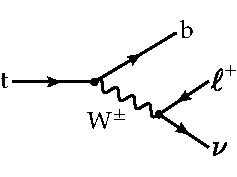
\includegraphics[scale=0.75]{figures/theory/t_decay.pdf}}\hspace{0.15\textwidth}
\subfloat[\label{fig:theory-top-whel-angle}]{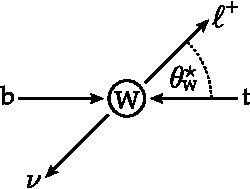
\includegraphics[scale=0.75]{figures/theory/whel.pdf}}
}

Potential scenarios of spin orientations at the $\mathrm{Wtb}$~vertex are presented in Fig.~\ref{fig:theory-top-whel-states} for longitudinal~($H=0$), left-handed~($H=-1$), and right-handed~($H=+1$) $\mathrm{W}$~bosons in the top quark rest frame. In the last scenario the conservation of angular momentum forces the $\mathrm{b}$~quark to be right-handed. This is however suppressed by the electroweak \gls{va} coupling structure leading to a nearly vanishing probability at \gls{lo}. It would vanish entirely only for massless $\mathrm{b}$~quarks since then the $\mathrm{b}$~quark helicity would be equal to its chirality~\cite{Bernreuther:2008ju}. The expected distributions per helicity state as a function of $\cos\theta^\star_\mathrm{W}$ are shown in Fig.~\ref{fig:theory-whel-distributions} together with the \gls{nnlo} \gls{sm} expectation of $\mathrm{F}_\mathrm{L}=0.311\pm0.005$, $\mathrm{F}_\mathrm{R}=0.0017\pm0.0001$, and $\mathrm{F}_{0}=0.687\pm0.005$~\cite{Czarnecki:2010gb}. The non-zero but small right-handed helicity fraction arises from the non-zero mass of the $\mathrm{b}$~quark and from the considered corrections beyond \gls{lo} to the vertices.
 
\myfigure{\label{fig:theory-top-whel-states}Scenarios of spin orientations at the $\mathrm{Wtb}$~vertex in the top quark rest frame. The right-handed $\mathrm{W}$~boson helicity~($H=+1$) is suppressed by the electroweak \gls{va} coupling structure which does not allow the right-handed $\mathrm{b}$~quark~(marked in red) to interact.}{
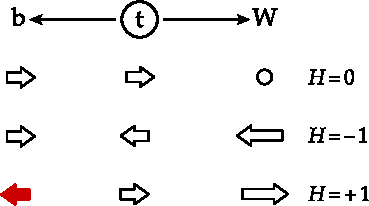
\includegraphics[scale=0.75]{figures/theory/whel_spins.pdf}
}
 
\myfigure{\label{fig:theory-whel-distributions}Distributions of the helicity angle for various W boson helicity scenarios. The \gls{sm} expectation at \gls{nnlo} is taken from Ref.~\cite{Czarnecki:2010gb}.}{
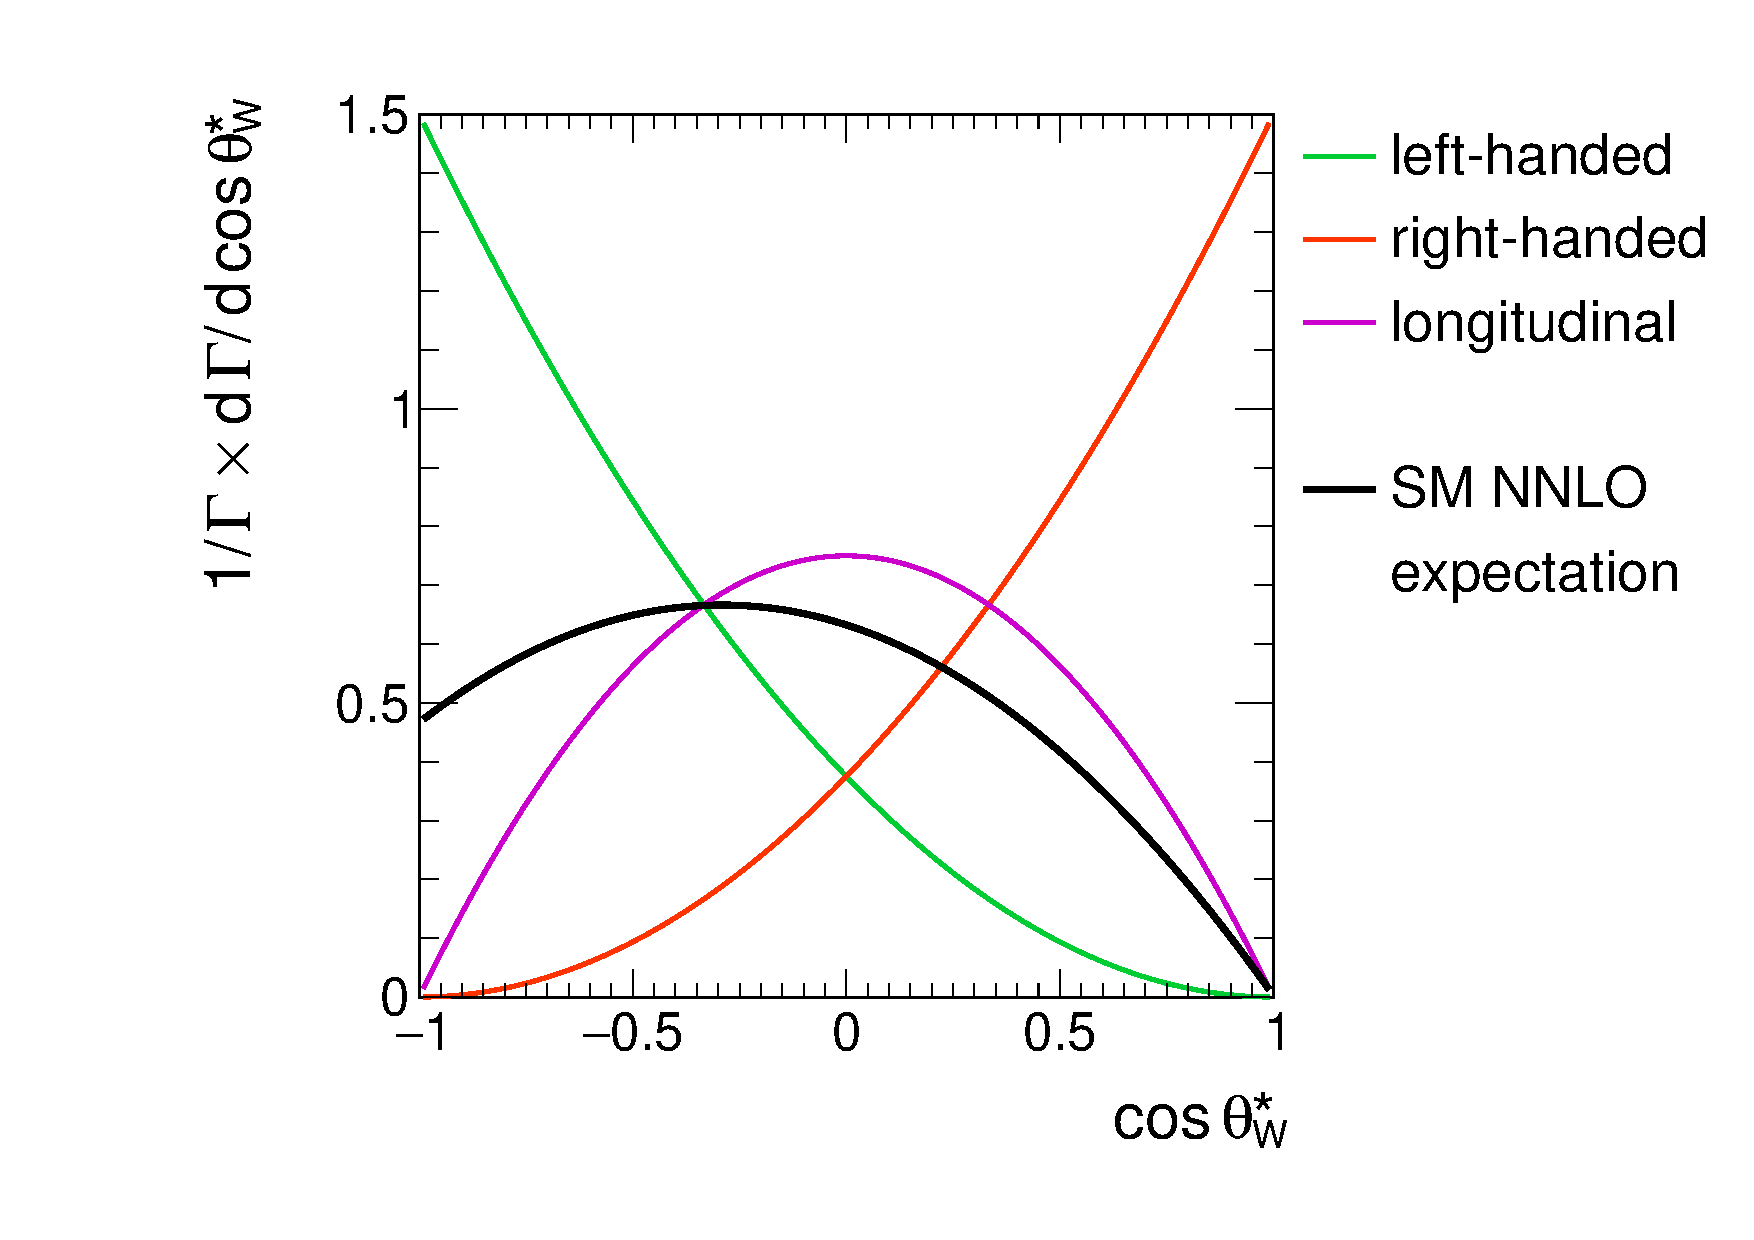
\includegraphics[width=0.49\textwidth]{figures/theory/whel_fractions.pdf}
}

For a general analysis of the top quark spin one introduces the so-called ``spin-analyzing power'', $\alpha_{X}\in[-1;\,1]$, of the decay product $X=\ell,\nu,\mathrm{W},\mathrm{b}$. It denotes the fraction of instances when the top quark spin is aligned along the momentum of the spin analyzer in the top quark rest frame. The calculated spin-analyzing powers at \gls{lo} and \gls{nlo} in the \gls{sm} are listed in Tab.~\ref{tab:theory-spin-powers}. Additionally, the spin-analyzing powers for $X=\mathrm{q},\mathrm{q}^\prime$ for $\mathrm{W}\to \mathrm{q}\,\mathrm{q}^\prime$ decays are provided where $\mathrm{q}$ ($\mathrm{q}^\prime$) denotes all up-type (down-type) quarks respectively. However, studying the top quark spin in those decays is experimentally very challenging since the original quark flavor of a jet and its origin in case of additional final state radiation are difficult to infer. The spin-analyzing powers flip their sign $\alpha_{X}=-\alpha_{\bar{X}}$ in the case of top antiquark decays for the corresponding particle or antiparticle. This holds also in \gls{bsm} scenarios inducing \gls{cp}-violation in the top quark sector~\cite{AguilarSaavedra:2010nx}.

\mytable{\label{tab:theory-spin-powers}Spin-analyzing power of the decay particles of the top quark. The values are taken from Ref.~\cite{AguilarSaavedra:2010nx} and references therein.}{
\begin{tabular}{|c| r@{.}l r@{.}l |}
\hline
decay product $X$           & \multicolumn{2}{c}{$\alpha_{X}^\mathrm{LO}$}      & \multicolumn{2}{c |}{$\alpha_{X}^\mathrm{NLO}$} \\
\hline
$\ell^{\rmplus}$            & \hspace{0.5cm}1&00\hspace{0.5cm}                  & \hspace{0.5cm}0&998\hspace{0.5cm} \\
$\nu$                       & -0&32                     & -0&33 \\
$\bar{\mathrm{q}}^\prime$ (down-type)   & 1&00          & 0&93 \\
$\mathrm{q}$~(up-type)      & -0&32                     & -0&31 \\
$\mathrm{b}$                & -0&41                     & -0&39 \\
$\mathrm{W}^{\rmplus}$      & 0&41                      & 0&39 \\
\hline
\end{tabular}
}

The charged lepton is a nearly perfect spin analyzer to study the top quark polarization. Its spin-analyzing power is even larger than that of its mother particle, the $\mathrm{W}$~boson, due to constructive (destructive) interference of the longitudinal and left-handed $\mathrm{W}$~boson helicity states in cases when the lepton is aligned (antialigned) with the top quark spin, respectively~\cite{Bernreuther:2008ju}. Simplified sketches of various spin orientations for longitudinal and left-handed $\mathrm{W}$~boson helicities are shown in Fig.~\ref{fig:theory-top-spin-orientations} demonstrating that the momentum of the charged antilepton in the top quark rest frame tends to be aligned along the top quark spin. Antialigned scenarios~(Figs.~\ref{fig:theory-top-spin-orientations-long-suppressed} and~\ref{fig:theory-top-spin-orientations-left-suppressed}) are suppressed by the \gls{va} coupling structure which does not allow right-handed particles~($\nu$) or left-handed antiparticles~($\ell^{\rmplus}$) to interact. Similar diagrams with reversed spin orientations are expected for top antiquarks.

\myfigure{\label{fig:theory-top-spin-orientations}Sketches of various spin orientations in top quark decays for (a,b)~longitudinal and (c,d)~left-handed $\mathrm{W}$~boson helicities. Suppressed spin orientations are marked in red.}{
\subfloat[]{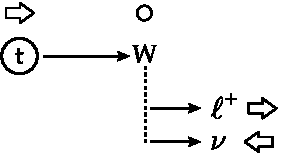
\includegraphics[scale=0.75]{figures/theory/top_spins_long_allowed.pdf}}\hspace{0.15\textwidth}
\subfloat[\label{fig:theory-top-spin-orientations-long-suppressed}]{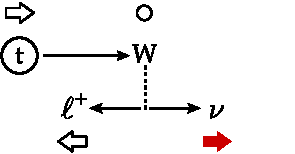
\includegraphics[scale=0.75]{figures/theory/top_spins_long_suppressed.pdf}}\\
\subfloat[]{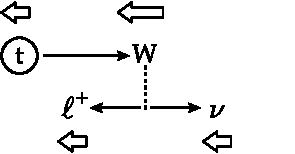
\includegraphics[scale=0.75]{figures/theory/top_spins_left_allowed.pdf}}\hspace{0.15\textwidth}
\subfloat[\label{fig:theory-top-spin-orientations-left-suppressed}]{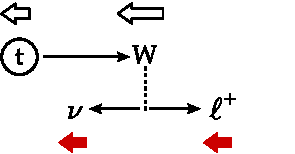
\includegraphics[scale=0.75]{figures/theory/top_spins_left_suppressed.pdf}}
}

%##############################################
\section{Pair production}
%##############################################
\label{sec:theory-ttbar-production}

The dominant mechanism producing top quarks at hadron colliders is top quark pair production through strong interactions via gluon~($gg\to\ttbar$) or quark fusion~($\mathrm{q}\bar{\mathrm{q}}\to\ttbar$). Figure~\ref{fig:theory-feynman-ttbar} shows the contributing Feynman diagrams at \gls{lo}. Especially the production channel via gluon fusion leads to a large cross section at the \gls{lhc} because of the steeply increasing gluon \gls{pdf} towards smaller momentum fractions. This channel contributes approximately $80\range90\%$ to the total cross section in the \gls{lhc} \acrlong{cm} energy regime of $7\range14~\TeV$~\cite{Olive:2016xmw}. The theoretical \ttbar cross sections in pp collisions at \acrlong{cm} energies of $8$ and $13~\TeV$, relevant for this thesis are listed in Tab.~\ref{tab:theory-ttbar-xsecs}. Those have been calculated at \gls{nnlo}+NNLL accuracy using the \textsc{Top++}\,2.0 program~\cite{Czakon:2011xx,Czakon:2013goa} assuming a top quark mass of $172.5~\GeV$. The \gls{pdf} uncertainty includes also the uncertainty on \as.

\myfigure{\label{fig:theory-feynman-ttbar}Feynman diagrams of \ttbar production at \gls{lo}: (a)~quark fusion; (b,c)~gluon fusion.}{
\subfloat[]{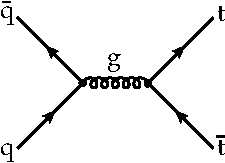
\includegraphics[scale=0.75]{figures/theory/qq2tt_1.pdf}}\hspace{0.03\textwidth}
\subfloat[]{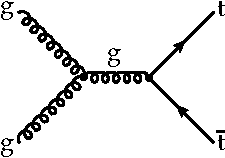
\includegraphics[scale=0.75]{figures/theory/qq2tt_2.pdf}}\hspace{0.03\textwidth}
\subfloat[]{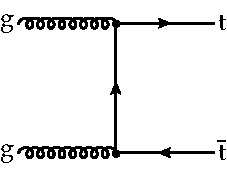
\includegraphics[scale=0.75]{figures/theory/qq2tt_3.pdf}}
}

\mytable{\label{tab:theory-ttbar-xsecs}Top quark pair production cross sections in per \acrlong{cm} energy.}{
\begin{tabular}{|c| r@{.}l@{}l@{$\,\mathrm{(scale)}$}l@{$\,\mathrm{(\gls{pdf})}~\pb$}l |}
\hline
\gls{cm}~energy       & \multicolumn{5}{c |}{cross section}     \\
\hline
$8~\TeV$     & $252$ & $9$ & ${}^{+6.4}_{-8.6}$ & $\pm11.7$ & \\
$13~\TeV$    & $831$ & $8$ & ${}^{+19.8}_{-29.2}$ & $\pm35.6$ & \\
\hline
\end{tabular}
}



%##############################################
\section{Single top quark production}
%##############################################
\label{sec:theory-single-top-production}

Besides the production in pairs, top quarks can be produced singly through electroweak interactions. At \gls{lo}, one can categorized the production into three main channels depending on the exchanged $\mathrm{W}$~boson and its virtuality $Q^{2}=-p_{\mu}p^{\mu}$. The corresponding Feynman diagrams are presented in Fig.~\ref{fig:theory-feynman-singletop}. Overall, the single-top-quark cross sections are smaller than for pair production due to the electroweak coupling strength $\aw<\as$. Additionally, the requirement of sea quarks~($\mathrm{b}$, $\bar{\mathrm{q}}$) in the initial states whose \glspl{pdf} increase less steeply at low momentum fractions compared to the gluon \gls{pdf} suppresses the cross sections further~(see Fig.~\ref{fig:theory-nnpdf-dist}).

\myfigure{\label{fig:theory-feynman-singletop}Feynman diagrams of electroweak single top quark production at \gls{lo} in the 5 flavor scheme.}{
\subfloat[\label{fig:theory-singletop-tch}$t$ channel]{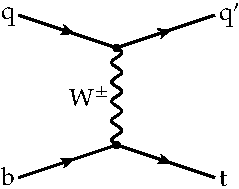
\includegraphics[scale=0.75]{figures/theory/ST_tch.pdf}}\hspace{0.05\textwidth}
\subfloat[\label{fig:theory-singletop-sch}$s$ channel]{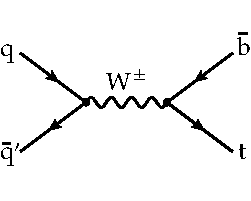
\includegraphics[scale=0.75]{figures/theory/ST_sch.pdf}} \\
\subfloat[\label{fig:theory-singletop-tWch}tW channel]{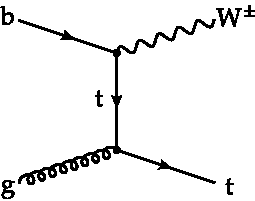
\includegraphics[scale=0.75]{figures/theory/ST_tWch2.pdf}\hspace{0.05\textwidth}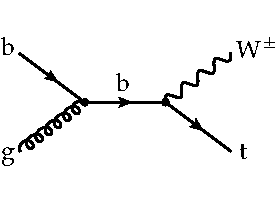
\includegraphics[scale=0.75]{figures/theory/ST_tWch.pdf}}
}

\begin{description}
\item[$\boldsymbol{t}$ channel] The production of single top quark in $t$-channel~(Fig.~\ref{fig:theory-singletop-tch}) has the highest cross section in $\mathrm{pp}$ collisions. Here, the virtuality of the $\mathrm{W}$~boson is found to be $Q^2>0$ and hence it is said to be ``space-like''. A characteristic feature of this mode is the additional spectator quark $q^\prime$ which recoils against the $\mathrm{W}$~boson and tends therefore being scattered fairly forward. In $t$-channel production, top quarks are produced roughly twice more often than top antiquarks reflecting the u~over d~valence quark ratio of the proton. This ratio depends however on the \acrlong{cm} energy. At higher energies, lower momentum fractions are reached at which the contributions from the valence quarks become less dominant. Hence the $\sigma(\mathrm{t})/\sigma(\bar{\mathrm{t}})$ charge ratio is sensitive to the \gls{pdf} of the proton.
\item[$\boldsymbol{s}$ channel] The mode with the smallest single-top-quark production cross section is via $s$ channel~(Fig.~\ref{fig:theory-singletop-sch}). This is because of the ``time-like'' $\mathrm{W}$~boson which has to have a large virtuality $Q^2<0$ to produce the heavier top quark. In various \gls{bsm} scenarios, the cross section of this process is expected to increase due to new heavy particles such as $\mathrm{W}^\prime$ or charged Higgs bosons which may even be produced on their mass shell, $p_{\mu}p^{\mu}-m^{2}=0$, and hence occur as a resonance.
\item[tW] The third mode is the production of a single top quark in association with a $\mathrm{W}$~boson~(Fig.~\ref{fig:theory-singletop-tWch}). Here, the $\mathrm{W}$~boson can be produced on-shell $Q^2=-m_\mathrm{W}^{2}$. It is commonly referred to as ``tW channel''. This process interferes at \gls{nlo} with \ttbar production which complicates its definition. In the \glshere{dr} scheme  diagrams with two resonant top quarks are subtracted from the amplitude whereas in the \glshere{ds} scheme the contribution from \ttbar is locally removed from the cross section~\cite{Tait:1999cf,1126-6708-2009-11-074}. The difference between both schemes lies in the treatment of the interference term which is kept in \gls{ds} but removed in \gls{dr}. A new approach is to combine both production modes and the inference between them into a process with a $\mathrm{W}^{\rmplus}\mathrm{W}^{\rmminus}\,\mathrm{b}\,\bar{\mathrm{b}}+X$ final state~\cite{Cascioli:2013wga} whose simulation is currently being studied.
\end{description}

The theoretical cross sections of the three single top quark production modes in pp collisions for center-of-mass energies of $8$ and $13~\TeV$, relevant for this thesis, are listed in Tab.~\ref{tab:theory-singletop-xsecs}. These have been calculated at \gls{nlo} in \gls{qcd} with the \HATHOR\,$2.1$ program~\cite{Aliev:2010zk,Kant:2014oha} using a top quark mass of $m_\mathrm{t}=172.5~\GeV$ while setting the factorization and renormalization scales to $\mu_\mathrm{R}=\mu_\mathrm{F}=m_\mathrm{t}$. The \gls{pdf} uncertainty includes also the uncertainty on \as.

\mytable{\label{tab:theory-singletop-xsecs}Single top quark cross sections per production mode and per \acrlong{cm} energy.}{
\begin{tabular}{|c| r@{.}l@{}l@{$\,\mathrm{(scale)}$}l@{$\,\mathrm{(\gls{pdf})}~\pb$}l  r@{.}l@{}l@{$\,\mathrm{(scale)}$}l@{$\,\mathrm{(\gls{pdf})}~\pb$}l |}
\hline
mode            & \multicolumn{5}{c }{$\sigma^{8~\TeV}$} & \multicolumn{5}{c |}{$\sigma^{13~\TeV}$}     \\
\hline
$t$ channel     & $84$ & $7$ & ${}^{+2.6}_{-1.7}$ & $\pm2.8$ &   \hspace{0.5cm}   & $217$ & $0$ & ${}^{+6.6}_{-4.6}$ & $\pm6.2$ & \\
tW channel      & $22$ & $4$ & $\pm0.6$ & $\pm1.4$ &      & $71$  & $7$ & $\pm1.8$ & $\pm3.4$ & \\
$s$ channel     & $5$  & $24$ & ${}^{+0.15}_{-0.12}$ & $\pm0.16$ &      & $10$  & $32$ & ${}^{+0.29}_{-0.24}$ & $\pm0.27$ & \\
\hline
\end{tabular}
}

Measurements of single-top-quark cross sections allow to extract a limit on the \gls{ckm} matrix element $\vtb$. If one assumes $|\vtd|^2+|\vts|^2\ll|\vtb|^2$ then the $\mathrm{t}\to\mathrm{bW}$ branching ratio can be approximated as

\begin{equation}
\mathcal{B}(\mathrm{t}\to\mathrm{bW})=\frac{|\vtb|^2}{\underbrace{|\vtd|^2+|\vts|^2}_{\ll|\vtb|^2}+|\vtb|^2}\approx 100\%\,.
\end{equation}

Hence, the cross section is independent of the top quark decay vertex and therefore directly proportional to $|f_\mathrm{L}\cdot\vtb|^2$. The form factor $f_\mathrm{L}$ is introduced to absorb potential contributions from \gls{bsm} physics that modify the left-handed coupling strength. It is $f_\mathrm{L}^\mathrm{SM}=1$ in the \gls{sm}. A measured single-top-quark cross section can then be used to extract the value of $|f_\mathrm{L}\vtb|$ as

\begin{equation}
|f_\mathrm{L}\vtb|=\sqrt{\frac{\sigma_\mathrm{measured}}{\sigma_\mathrm{theory}}}\,.
\end{equation}

It should be noted that for this interpretation of single-top-quark cross sections, no assumptions on the number of quark generations and subsequently no unitarity of the \gls{ckm} matrix is required.



%##############################################
\section{Polarization in \textit{t}-channel single-top-quark production}
%##############################################
\label{sec:theory-t-channel-polarization}

The \gls{sm} predicts that top quarks are produced highly polarized in $t$~channel since there are only electroweak interactions with a \gls{va} coupling structure involved at \gls{lo}~\cite{Bernreuther:2008ju}. A new \gls{bsm} physics model may however lead to a depolarization by altering the coupling structure effectively through new production vertices and/or higher order corrections. The differential cross section can be parametrized as

\begin{equation}
\frac{\mathrm{d}\sigma}{\sigma\cdot\mathrm{d}\cos\theta^\star_{X}}=\frac{1}{2}\,\Big(1+\mathrm{P}_\mathrm{t}\cdot\alpha_{X}\cdot\cos\theta^\star_{X}\Big)\,,
\end{equation}

where $\mathrm{P}_\mathrm{t}$ denotes the polarization along a given axis and $\alpha_{X}$ the spin-analyzing power with respect to decay product $X$. The polarization angle

\begin{equation}
\cos\theta^\star_{X}=\frac{\vec{s}_\mathrm{t}\cdot \vec{p}_{X}^\scriptn{\mathrm{(t)}}}{\big|\vec{s}_\mathrm{t}\big|\cdot\big|\vec{p}_{X}^\scriptn{\mathrm{(t)}}\big|}
\end{equation}

is taken between the spin analyzer $X$ in the top quark rest frame and a suitable spin quantization axis $\vec{s}_\mathrm{t}$. A potential spin axis is given in the helicity basis where the top quark momentum in the partonic \acrlong{cm} system is chosen, $\vec{s}_\mathrm{t}^\scriptn{\,\mathrm{hel.}}=\vec{p}_\mathrm{t}^\scriptn{\mathrm{(tq)}}$. However, this system cannot be reconstructed unambiguously beyond \gls{lo} when additional \glshere{isr} or \glshere{fsr} occurs. An alternative axis is motivated in Fig.~\ref{fig:theory-t-channel-prod-decay} where a sketch of spin orientations in the top quark rest frame for $t$-channel production and decay is shown. There exists a symmetry between a down-type spectator quark on the production side and the charged antilepton on the decay side leading to a correlation between their momentum directions and the intermediate top quark spin. This suggests to take the spectator quark momentum in the top quark rest frame as the spin quantization axis, $\vec{s}_\mathrm{t}=\vec{p}_{\mathrm{q}^\prime}^\scriptn{\mathrm{(t)}}$. At \gls{lo}, this axis would coincide with the axis in helicity basis since the top quark and the spectator quark are back-to-back in the \acrlong{cm} system~\cite{Schwienhorst:2010je}. A high degree of polarization can therefore be expected. This is further motivated by the fact that the charged lepton is a nearly perfect spin analyzer and thus the down-type spectator quark is a good spin analyzer as well because of the depicted symmetry. Higher-order corrections however dilute this symmetry somewhat as also expected from Tab.~\ref{tab:theory-spin-powers} where a slightly lower spin-analyzing power for the down-type quark compared to the charge lepton at \gls{nlo} is expected. 

\myfigure{\label{fig:theory-t-channel-prod-decay}Sketch of spin orientations in $t$-channel single-top-quark production and decay. The figure has been inspired from Ref.~\cite{Schwienhorst:2010je}.}{
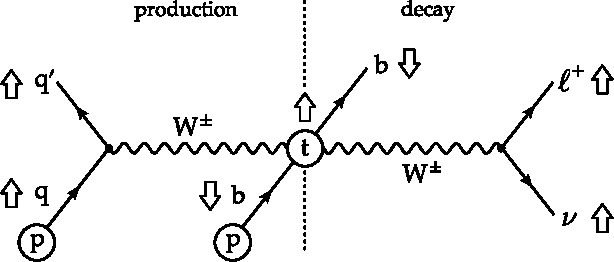
\includegraphics[scale=0.75]{figures/theory/t-channel-prod-decay.pdf}
}

A crucial ingredient which is still missing in this argumentation is the fact that the spectator quark has to be of down-type flavor. This is only true in about $80\%$ for $t$-channel top quark production but only in $31\%$ of all cases for top antiquark production. Here, the down-type quark is found with a probability of $69\%$ in the initial state instead. However, the spectator quark is only mildly deflected after recoiling against the $\mathrm{W}$~boson. It is therefore still sufficiently close to the direction of the down-type quark momentum resulting in a high degree of polarization nonetheless~\cite{Bernreuther:2008ju}.

The expect top quark polarizations have been calculated at $7~\TeV$ and are listed in Tab.~\ref{tab:theory-singletop-sm-polarization} at \gls{lo} and \gls{nlo}. The combined polarization for top quark and antiquark is calculated using a weighted sum with the corresponding cross sections as weights\footnote{The expected single-top-quark cross sections at $7~\TeV$ are $\sigma(\mathrm{t})=41.8^{+1.8}_{-1.5}~\pb$ and $\sigma(\bar{\mathrm{t}})=22.0^{+1.3}_{-1.2}~\pb$. These are calculated with the same setup as used for Tab.~\ref{tab:theory-singletop-xsecs}}. At $8~\TeV$, a similar polarization of $|\mathrm{P}_{\mathrm{t}+\bar{\mathrm{t}}}^\mathrm{8~\TeV}|=0.88$ is expected using simulated events from the \gls{nlo} generator \textsc{Powheg}~\cite{Khachatryan:2015dzz}.

\mytable{\label{tab:theory-singletop-sm-polarization}Expected polarizations of top quarks and top antiquarks in $t$-channel single-top-quark production at $7~\TeV$. The values are taken from Ref.~\cite{Schwienhorst:2010je}.}{
\begin{tabular}{|c| r@{.}l r@{.}l r@{.}l|}
\hline
            & \multicolumn{2}{c}{$\mathrm{P}_\mathrm{t}^\mathrm{\,7\,\TeV}$} & \multicolumn{2}{c}{$\mathrm{P}_{\bar{\mathrm{t}}}^\mathrm{\,7\,\TeV}$} & \multicolumn{2}{c|}{$|\mathrm{P}_{\mathrm{t}+\bar{\mathrm{t}}}^\mathrm{\,7\,\TeV}|$}     \\
\hline
\hline
\gls{lo}    & \hspace{0.5cm}0&99\hspace{0.5cm} & \hspace{0.5cm}-0&93\hspace{0.5cm}       & \hspace{0.5cm}0&95\hspace{0.5cm}          \\
\gls{nlo}   & 0&91                             & -0&86                                   & 0&88          \\
\hline
\end{tabular}
}

The high polarization of the top quark along the spectator quark momentum allows also to extend the $\mathrm{W}$~boson polarization with two additional axes. Figure~\ref{fig:theory-ext-whel} shows the construction procedure. The top quark spin is approximated by the spectator quark momentum. Then the normal and transverse axes are defined as 

\begin{subequations}
\begin{align}
\vec{\mathrm{N}}&=\vec{p}_{\mathrm{q}^\prime}^{\mathrm{(t)}}\times\vec{p}_{\mathrm{W}}^{\mathrm{(t)}}\qquad\text{(normal axis)} \\
\vec{\mathrm{T}}&=\vec{p}_{\mathrm{W}}^{\mathrm{(t)}}\times \vec{\mathrm{N}}\qquad\text{(transverse axis)}.
\end{align}
\end{subequations}

\myfigure{\label{fig:theory-ext-whel}Extended $\mathrm{W}$~boson polarization axes in $t$-channel single-top-quark production and decay: $\mathrm{N}=\text{normal axis}$; $\mathrm{T}=\text{transverse axis}$.}{
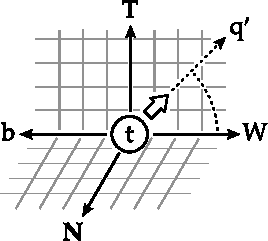
\includegraphics[scale=0.75]{figures/theory/ext_whel.pdf}
}

The differential cross section as a function of the polarization angles with these new axes takes the same functional form as in Eq.~\ref{eq:theory-diff-whel-fractions}. However, the corresponding polarization fractions $\mathrm{F}_\mathrm{L}^\mathrm{N,T}$, $\mathrm{F}_\mathrm{0}^\mathrm{N,T}$, and $\mathrm{F}_\mathrm{R}^\mathrm{N,T}$ are probing here different aspects of the coupling structure. In particular, the left- and right-handed polarization along $\vec{\mathrm{N}}$ are sensitive to potential \gls{cp}-violation~\cite{AguilarSaavedra:2010nx}. Since the top quark is not fully polarized along the spectator quark momentum, the  polarization fractions are modified as

\begin{subequations}
\begin{align}
\tilde{\mathrm{F}}_\mathrm{R}^\mathrm{N,T}&=\frac{1+\mathrm{P}_\mathrm{t}}{2}\cdot\mathrm{F}_\mathrm{R}^\mathrm{N,T}+\frac{1-\mathrm{P}_\mathrm{t}}{2}\cdot\mathrm{F}_\mathrm{L}^\mathrm{N,T}, \\
\tilde{\mathrm{F}}_\mathrm{L}^\mathrm{N,T}&=\frac{1+\mathrm{P}_\mathrm{t}}{2}\cdot\mathrm{F}_\mathrm{L}^\mathrm{N,T}+\frac{1-\mathrm{P}_\mathrm{t}}{2}\cdot\mathrm{F}_\mathrm{R}^\mathrm{N,T}, \\
\tilde{\mathrm{F}}_\mathrm{0}^\mathrm{N,T}&=\mathrm{F}_\mathrm{0}^\mathrm{N,T}\,.
\end{align}
\end{subequations}


%##############################################
\section{Flavor schemes}
%##############################################

In single-top-quark production via $t$ channel, a $\mathrm{b}$~quark is required in the initial state. There are two different ways called 4 and 5~\glshere{fs} to treat the $\mathrm{b}$~quark in theoretical calculations. They differ in the number of quark flavors which are included within the proton~\gls{pdf}. Figure~\ref{fig:theory-flavorscheme} shows a representative Feynam diagram where in 4~\gls{fs} the $\mathrm{b}$~quark originates from gluon splitting and is not part of the \gls{pdf}. In 5~\gls{fs} this splitting is resumed into the \gls{pdf} instead.

\myfigure{\label{fig:theory-flavorscheme}Feynman diagram at \gls{lo} for $t$-channel single-top-quark production in 4 and 5~\glsreset{fs}\gls{fs}. The dashed lines denote where the partonic initial state begins.}{
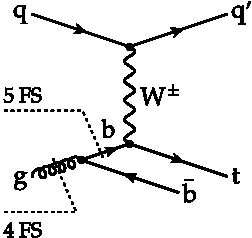
\includegraphics[scale=0.75]{figures/theory/flavorscheme.pdf}
}

Since the $\mathrm{b}$~quark mass of $m_\mathrm{b}\approx4.2~\GeV$ is higher than the mass of the proton, $m_\mathrm{p}\approx1~\GeV$, the 4~\gls{fs} seems more natural at first glance. The $\mathrm{b}$~quark is treated as a heavy quark state that decouples completely from the \as and \gls{pdf} evolutions through renormalization and the DGLAP equation, respectively. However, this approach results in terms proportional to $\log(Q^2/m_\mathrm{b}^2)$ arising from the intermediate $\mathrm{b}$~quark propagator which may prohibit the convergence of perturbative calculations at high momentum transfers $Q$. In this case, such terms together with the $g\to\mathrm{b}\bar{\mathrm{b}}$ splitting function can be absorbed into a \gls{pdf} for the $\mathrm{b}$~quark instead~\cite{Maltoni:2012pa}.

Both schemes are valid approaches for calculating observables. The difference at fixed order stems from the energy scale at which a process is described. Both approaches will converge at sufficiently high orders. This is demonstrated in Fig.~\ref{fig:theory-t-channel-xsec-fs} where the $t$-channel single-top-quark cross section at $14~\TeV$ as a function of the renormalization and factorization scale is depicted. The dashed curves show the \gls{lo} predictions in 4~and 5~\gls{fs} respectively which are far apart. Their opposite behavior originates from the running of coupling constant \as in the 4~\gls{fs} versus the scale dependence of the $\mathrm{b}$~quark \gls{pdf} in the 5~\gls{fs}~\cite{Maltoni:2012pa}. They approach the \gls{nlo} prediction only at low (large) scales for 4~\gls{fs} (5~\gls{fs}) respectively. On the other hand, the \gls{nlo} predictions start to converge already at a scale choice of $\mu\approx m_\mathrm{t}/2$ for this process.

\myfigure{\label{fig:theory-t-channel-xsec-fs}Single-top-quark cross section in $t$ channel for top quarks at $14~\TeV$ as a function of the renormalization and factorization scale $\kappa=\mu/m_\mathrm{t}$. The predicted cross sections calculated in 4~and 5~\gls{fs} at \gls{lo} and \gls{nlo} are displayed. The figure is taken from Ref.~\cite{Maltoni:2012pa}}{
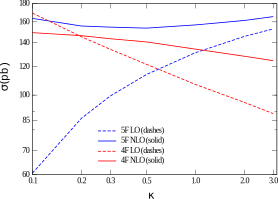
\includegraphics[scale=0.9]{figures/theory/t-channel-xsec-fs}
}

Predictions of differential distributions are also affected by the flavor scheme choice. Ratios of 4~\gls{fs} over 5~\gls{fs} differential $t$-channel cross sections at \gls{nlo} as a function of the transverse momentum and pseudo rapidity with respect to the top quark and spectator jet are shown in Fig.~\ref{fig:theory-t-channel-xsec-fs-diff}. The differences between both schemes are found to be around the $10~\%$ level~\cite{Campbell:2009ss}. In particular, the top quark \pt displays here an almost linear increasing ratio.

\myfigure{\label{fig:theory-t-channel-xsec-fs-diff}Ratio of 4~\gls{fs}~($\sigma^{2\to3}$) over 5~\gls{fs}~($\sigma^{2\to2}$) differential single-top-quark cross sections in $t$ channel for top quarks at $14~\TeV$ as a function of (a)~the transverse momentum and (b)~the pseudo rapidity of the top quark and light (spectator) jet. The figures are taken from Ref.~\cite{Campbell:2009ss}}{
\subfloat[]{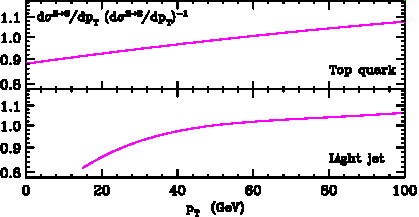
\includegraphics[scale=1]{figures/theory/t-channel-fs-diff-pt.pdf}}\\
\subfloat[]{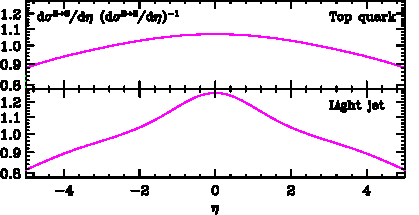
\includegraphics[scale=1]{figures/theory/t-channel-fs-diff-eta.pdf}}
}


%##############################################
\section{Anomalous couplings}
%##############################################

Direct searches for \gls{bsm} physics can be viewed as a top-down approach. The starting point is marked by a well-defined and usually \gls{uv}-complete \gls{bsm} theory. Experimentally, one is then interested to detect additional events originating from a new process within such a theory. Exemplary models are the \glshere{mssm}~(reviewed in Ref.~\cite{Csaki:1996ks}) or the \glshere{2hdm}~\cite{Branco:2011iw}. Since no signal has been found yet it may be that the energy scale at which a \gls{bsm} process becomes significant is not accessible in direct searches. Nonetheless, new particles or interactions can contribute higher-order corrections to processes within the \gls{sm} already at low energies. An example is the observation of the rare $\mathrm{B}^{0}_\mathrm{s}\to\mu\mu$ decay~\cite{CMS:2014xfa} which can be altered by contributions from e.g. the \gls{mssm}. This motivates a model-independent bottom-up approach where observables of the \gls{sm} are measured with great precision and compared to their expectation. Any deviations can then be interpreted within multiple new theories.

The idea of a bottom-up approach is depicted in Fig.~\ref{fig:theory-t-channel-eff} for some exemplary \gls{uv}-complete theory contributing to single top quark production through a new heavy scalar particle $\chi$. If the new particle has a sufficiently high mass it would not be possible to observe it as a new resonance in $s$~channel. However, the shown production of single top quarks would be altered through additional contributions from this new process. At energies $q\ll m_{\chi}$ it would mimic a 4-fermion contact interaction with a simple scalar coupling structure. The \mbox{\gls{sm}+\gls{bsm}} cross section of this process may still correspond to the one expected from the \gls{sm} alone by fine-tuning the \gls{sm} and \gls{bsm} couplings correspondingly. However, since this new process has a scalar coupling structure it manifests itself as a deviation from the expected \gls{va} coupling structure. Differential cross section measurements and related observables like the top quark polarization can then be used to probe for such anomalous couplings at the production vertex.

\myfigure{\label{fig:theory-t-channel-eff}Feynman diagram of potential \gls{bsm} physics contributing to single-top-quark production via flavor-changing neutral current interaction. At low energies $p\ll m_\chi$ the propagator in (a) can be approximated as an anomalous 4-fermion coupling~(b).}{
\subfloat[\label{fig:theory-t-channel-chi-uv}$t$~channel]{\parbox{0.35\textwidth}{\centering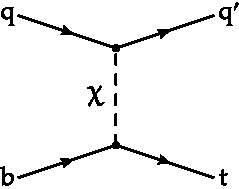
\includegraphics[scale=0.75]{figures/theory/t-channel-chi.pdf}\\$\propto \frac{g^2}{p^2-m^{2}_{\chi}}$}}
\subfloat[\label{fig:theory-t-channel-eff-ir}effective interaction]{\parbox{0.35\textwidth}{\centering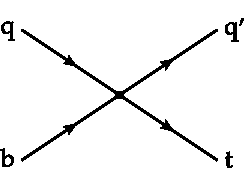
\includegraphics[scale=0.75]{figures/theory/t-channel-contact.pdf}\\$\propto \frac{g^2}{m^{2}_{\chi}}$}}
}

Such deviations from the \gls{sm} coupling structure can be characterized in the framework of effective field theories~(\glsplmark{eft}) in a model-independent manner. Those can be derived using an \glshere{ope} as first proposed in Ref.~\cite{Wilson:1972ee}. Here, products of operators are expanded as

\begin{equation}
{O}_{1}(x_{1})\ldots {O}_{n}(x_{n})=\sum_{i}c_{1\ldots n}^{i}(x_{1},\ldots x_{n})\cdot{O}_{i}^\mathrm{eff}(x_{n})\,,
\end{equation}

where $O_{i}^\mathrm{eff}$ denote effective operators and $c^{i}$ are the so-called Wilson coefficients. The expansion is applicable if $x_{1\ldots n-1}$ are close to $x_n$, i.e. only the low energy limit of a \gls{uv}-complete theory is relevant. Otherwise, unitarity can be violate if the energy scale of a process within the \gls{eft} approaches the scale of the concrete \gls{bsm} theory as discussed in Sec.~\ref{sec:theory-observables}. In the example above this would be the case when the momentum transfer $q$ approaches $m_\chi$. Here, the \gls{eft} approach becomes invalid.

One can extend the Lagrangian of the \gls{sm}, which contains only operators up to dimension-four, into an effective one as

\begin{equation}
\mathcal{L}^\mathrm{eff}=\mathcal{L}^\mathrm{\gls{sm}}_\mathrm{(4)}+\frac{1}{\Lambda}\sum_{i}c_{i}^\mathrm{(5)}{O}_{i}^\mathrm{(5)}+\frac{1}{\Lambda^{2}}\sum_{i}c_{i}^\mathrm{(6)}{O}_{i}^\mathrm{(6)}+\mathcal{O}\left(\frac{O^\mathrm{(7)}}{\Lambda^3}\right)\,,
\end{equation}

where new effective operators of dimension-five and -six have been added. Those are however suppressed by inverse powers of the new physics scale $\Lambda$. This approach leads to 59 independent operators of dimension-six when requiring gauge invariance and baryon number conservation~\cite{Grzadkowski:2010es}. The only operator of dimension-five is

\begin{equation}
\mathcal{L}^\mathrm{eff.}_\mathrm{(5)}=\frac{1}{\Lambda}c^{ij}_{\nu\nu}\Big({\mathrm{E}}^{c}_{\mathrm{L},i}\tilde{\phi}\Big)^\mathrm{T}\Big(\vec{\mathrm{E}}_{\mathrm{L},j}\tilde{\phi}\Big)+\mathrm{\gls{hc}},\qquad \tilde{\phi}_{a}=\epsilon_{ab}\phi_{b}
\end{equation}

which can be used to introduce neutrino masses and mixing after electroweak symmetry breaking\footnote{This assumes Majorana neutrinos. The coefficients $c^{ij}(v^2/\Lambda)$ can be interpreted as mass mixing matrix for neutrinos similar to the \gls{ckm} matrix for quarks. The superscript $c$ stands for charge conjugation.}. Only a subset of operators are relevant in the top quark sector~\cite{AguilarSaavedra:2008zc}. In particular, the following operators contribute to the $\mathrm{Wtb}$~vertex


\begin{subequations}
\begin{align}
\mathcal{L}^\mathrm{eff.}_\mathrm{Wtb}&=\mathcal{L}^\mathrm{SM}_\mathrm{Wtb}+\frac{1}{\Lambda^2}\Big(c_{\phi\mathrm{q}}^{33}O_{\phi\mathrm{q}}^{33}+c_{\phi\phi}^{33}O_{\phi\phi}^{33}+c_{\mathrm{dW}}^{33}O_{\mathrm{dW}}^{33}+c_{\mathrm{uW}}^{33}O_{\mathrm{uW}}\Big)+\mathrm{\gls{hc}} \\ 
O_{\phi\mathrm{q}}^{33}&=i\Big(\phi^\dagger\omega_{a}\mathrm{D}_\mu\phi\Big)\Big(\bar{\mathrm{Q}}_\mathrm{L}^{3}\gamma^{\mu}\omega^{a}\mathrm{Q}_\mathrm{L}^{3}\Big)\,,\qquad
O_{\phi\phi}^{33}=i\Big(\tilde{\phi}^\dagger\mathrm{D}_\mu\phi\Big)\Big(\bar{\mathrm{u}}_\mathrm{R}^{3}\gamma^{\mu}\mathrm{d}_\mathrm{R}^{3}\Big)\,,\\
O_{\mathrm{dW}}^{33}&=\Big(\bar{\mathrm{Q}}_\mathrm{L}^{3}\sigma^{\mu\nu}\omega_{a}\mathrm{d}_\mathrm{R}^{3}\Big)\phi\,\mathrm{W}^{a}_{\mu\nu}\,,\qquad
O_{\mathrm{uW}}=\Big(\bar{\mathrm{Q}}_\mathrm{L}^{3}\sigma^{\mu\nu}\omega_{a}\mathrm{u}_\mathrm{R}^{3}\Big)\tilde{\phi}\,\mathrm{W}^{a}_{\mu\nu}\,,
\end{align}
\label{eq:theory-eft-lagrangian-operators}
\end{subequations}

where $D_\mu$ denotes the covariant derivative~(Eq.~\ref{eq:theory-phi-codev}) and the quark field indices refer to the third generation following the notation of Eqs.~\ref{eq:theory-su2-doublets} and~\ref{eq:theory-su2-singlets}. Anomalous couplings can be introduced after electroweak symmetry breaking which absorb all constant terms including $c_{i}(v^2/\Lambda^2)$. One obtains

\begin{align}
\mathcal{L}^\mathrm{eff.}_\mathrm{Wtb}=&-\frac{g}{\sqrt{2}}\bar{\mathrm{b}}\gamma^{\mu}\big(\mathrm{V}_\mathrm{L}\mathrm{P}_\mathrm{L}+\mathrm{V}_\mathrm{R}\mathrm{P}_\mathrm{R}\big)\mathrm{t}\mathrm{W}_\mu^{\rmminus}\nonumber\\
&-\frac{g}{\sqrt{2}}\bar{\mathrm{b}}\frac{i\sigma^{\mu\nu}q_\nu}{m_\mathrm{W}}\big(\mathrm{g}_\mathrm{L}\mathrm{P}_\mathrm{L}+\mathrm{g}_\mathrm{R}\mathrm{P}_\mathrm{R}\big)\mathrm{t}\mathrm{W}_\mu^{\rmminus}+\mathrm{\gls{hc}}\,,\label{eq:theory-wtb-eff-anomcouplings}
\end{align}

where $\mathrm{V}_\mathrm{L,R}$ and $\mathrm{g}_\mathrm{L,R}$ denote the vector- and tensor-like anomalous couplings respectively. In the \gls{sm}~(Eq.~\ref{eq:theory-qqW-int}) there exists only a vector-like, left-handed coupling $\mathrm{V}_\mathrm{L}=\mathrm{V}_\mathrm{tb}$ whereas the other couplings vanish $\mathrm{V}_\mathrm{R}=\mathrm{g}_\mathrm{L}=\mathrm{g}_\mathrm{R}=0$.

The operator $O_\mathrm{qW}^{ij}$ is missing in Eq.~\ref{eq:theory-eft-lagrangian-operators}. Its contribution can be mostly absorbed by the other operators as

\begin{align}
\mathcal{L}_\mathrm{qW}&=\frac{1}{\Lambda^2}c^{ij}_\mathrm{qW}O_\mathrm{qW}^{ij}=\frac{1}{\Lambda^2}c^{ij}_\mathrm{qW}\Big(\bar{\mathrm{Q}}_{\mathrm{L},i}\gamma^{\mu}\omega_{a}D^\nu\mathrm{Q}_{\mathrm{L},j}\Big)\mathrm{W}_{\mu\nu}^{a}+\mathrm{\gls{hc}}\nonumber\\
&\supset\big(\text{terms }\propto\mathcal{L}_\mathrm{Wtb}^\mathrm{eff.}\big)~+~\frac{g\,\mathrm{Re}(c_\mathrm{qW})}{\Lambda^2}\big(\bar{\mathrm{b}}\gamma^{\mu}\mathrm{P}_\mathrm{L}\mathrm{t}\big)\big(\bar{\mathrm{q}}\gamma_\mu\mathrm{P}_\mathrm{L}\mathrm{q}^\prime\big)+\mathrm{\gls{hc}}\,,\label{eq:theory-4q-eff-anomcouplings}
\end{align}

where however a four-fermion contact interaction term remains~\cite{Bach:2012fb}. This interaction cannot contribute to top quark production and decays via a $\mathrm{Wtb}$~vertex directly which is why it is usually left out of Eqs.~\ref{eq:theory-eft-lagrangian-operators} and~\ref{eq:theory-wtb-eff-anomcouplings}. However, the four-fermion vertex should not be neglected when studying in particular single top quark production. Here, it can contribute a $\mathrm{udbt}$~vertex (similar to Fig.~\ref{fig:theory-t-channel-eff-ir}) as an addition to the $\mathrm{Wud}\text{+}\mathrm{Wtb}$~vertices which e.g. occur in the production via $t$~channel.

To constrain anomalous couplings from experimental data, various (pseudo) observables are proposed in literature~\cite{AguilarSaavedra:2010nx,Aguilar-Saavedra:2014eqa,Bernreuther:2015yna}. A few of them are the inclusive single-top-quark cross sections, the W~boson helicity fractions~(Sec.~\ref{sec:theory-top-quark-decay}), and the top quark polarization in $t$~channel~(Sec.~\ref{sec:theory-t-channel-polarization}).

\todo{mention topfit}

%##############################################
\section{Experimental results}
%##############################################
\label{sec:theory-exp-results}

To conclude this chapter, a brief overview of experimental results in the top quark sector are presented.

An overview of inclusive \ttbar cross section measurements at center-of-mass energies of 5\footnote{The 5~\TeV dataset was recorded in autumn 2015. It stems from a special pp collision run with low pileup which is used as a reference for measurements using heavy ion collisions.}, 7, 8, and 13~\TeV are shown in Fig.~\ref{fig:theory-lhc-ttbar-xsec} and compared to the theoretical \gls{nnlo}+\gls{nnll} prediction. Currently, the most precise result at 13~\TeV by \gls{cms} has been obtained from events with one electron or muon and at least one jet. The inclusive cross section is measured as $\sigma({\ttbar})=835\pm3\,\mathrm{(stat)}\pm23\,\mathrm{(syst)}\pm23\,\mathrm{(lumi)}~\pb$ which agrees well with the \gls{sm} prediction~(Tab.~\ref{tab:theory-ttbar-xsecs}). From the cross section the pole mass of the top quark is estimated to be $m_\mathrm{t}=172.3^{+2.7}_{-2.3}~\GeV$~\cite{CMS-PAS-TOP-16-006}.

Measurements of inclusive single-top-quark production in $t$, tW, and $s$~channel at 7, 8, and 13~\TeV are summarized and compared to the theoretical \gls{nlo} predictions in Fig.~\ref{fig:theory-lhc-st-xsec}. For $s$~channel, mostly only upper limits on the cross sections are depicted. The only evidence so far has been obtained by \gls{atlas} with a significance of $3.2$ standard deviations~\cite{Aad:2015upn}. All of these cross section measurements can be used to estimate the absolute value of the \gls{ckm} matrix element $\vtb$ as detailed in Sec.~\ref{sec:theory-single-top-production}. The results are presented in Fig.~\ref{fig:theory-lhc-vtb}. The currently most precise estimation of $\vtb$ stems from a combination of $t$-channel single-top-quark cross section measurements at 7 and 8~\TeV by \gls{cms} resulting in $|f_\mathrm{L}\vtb|=0.998\pm0.038\,\mathrm{(exp)}\pm0.016\,\mathrm{(theo)}$. This yields a limit of $|\vtb|>0.92$ at 95\%~\gls{cl} when assuming $f_\mathrm{L}=1$ and $|\vtb|<1$.


\myfigure[p]{Overview of inclusive (a)~top quark pair and (b)~single top quark cross section measurements by the \gls{atlas}~and \gls{cms}~collaborations at various center-of-mass energies. The figures are taken from the TopLHC working group.}{
\subfloat[\label{fig:theory-lhc-ttbar-xsec}]{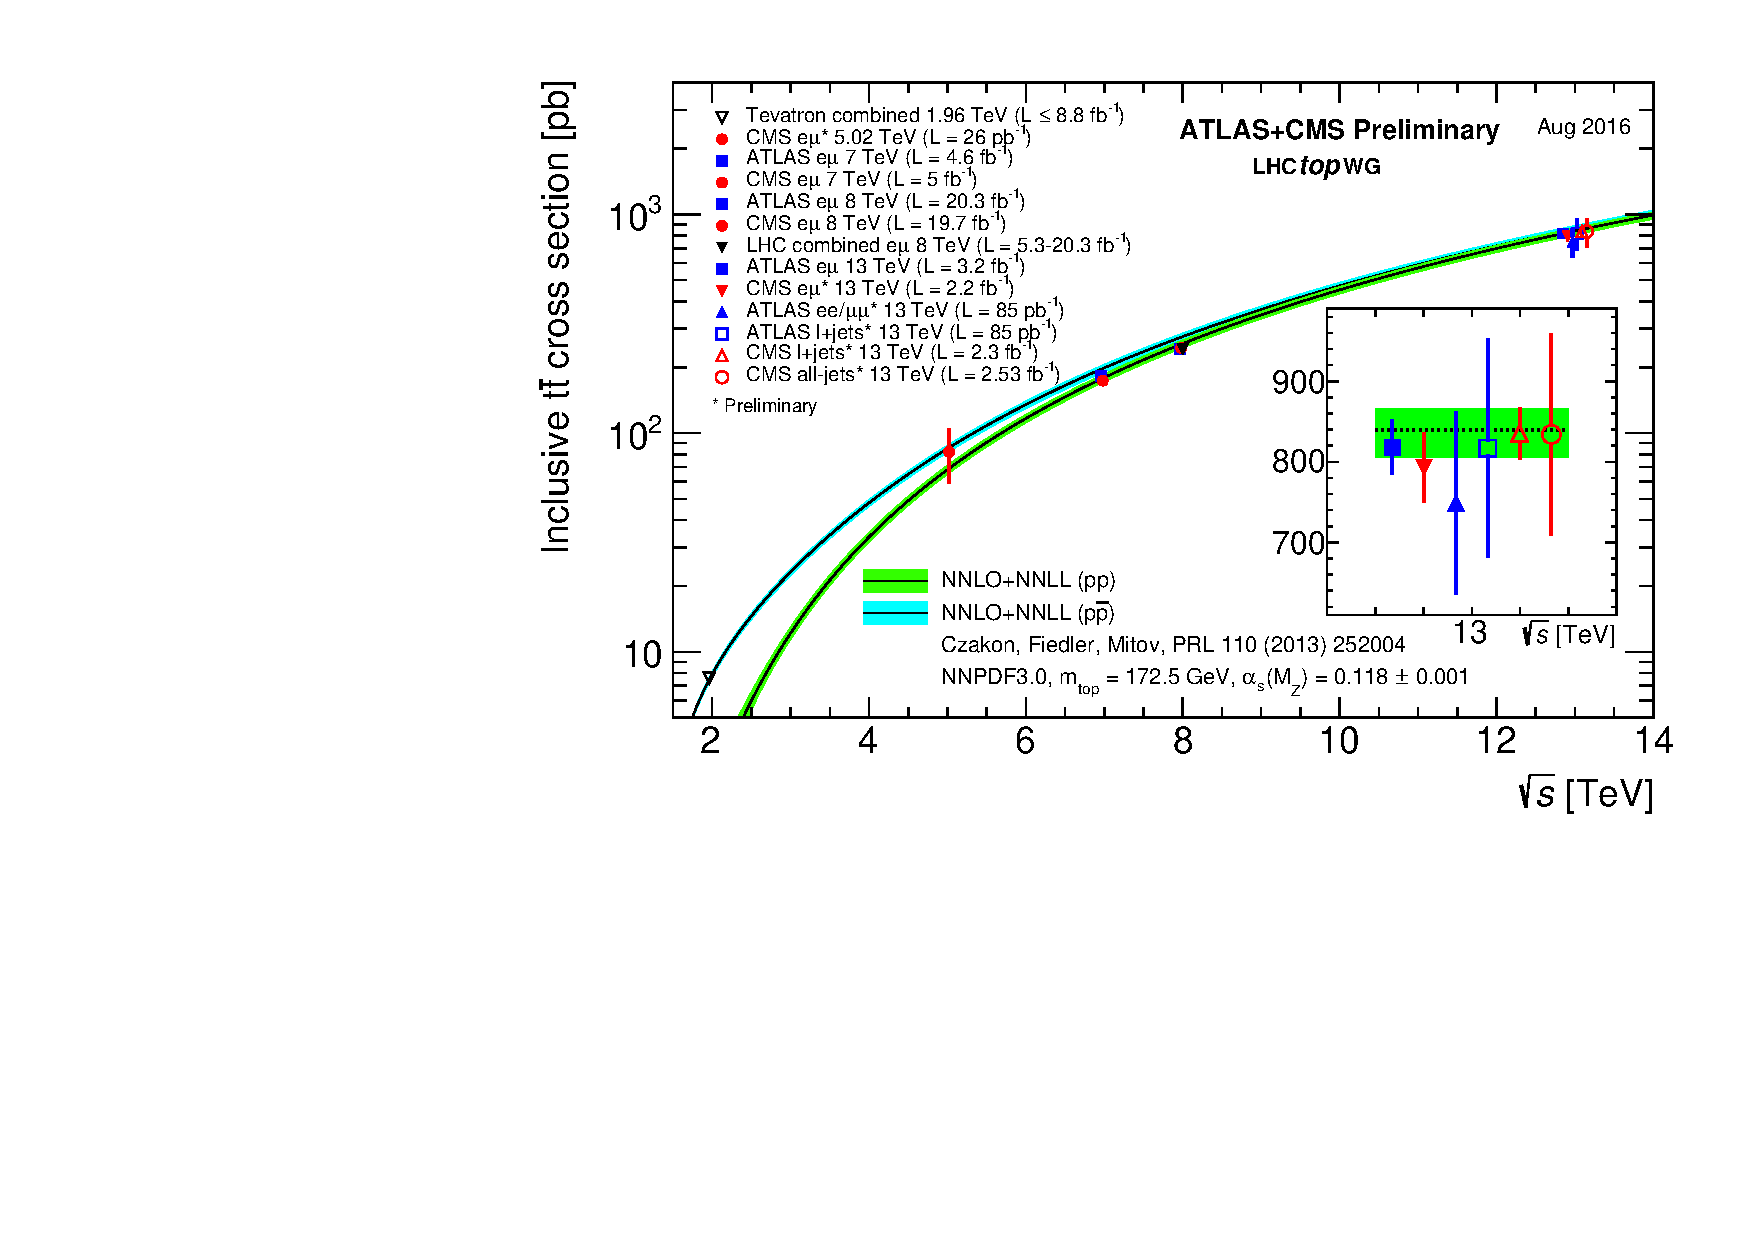
\includegraphics[width=0.96\textwidth]{figures/theory/LHC_ttxsec_sqrts.pdf}}\\
\subfloat[\label{fig:theory-lhc-st-xsec}]{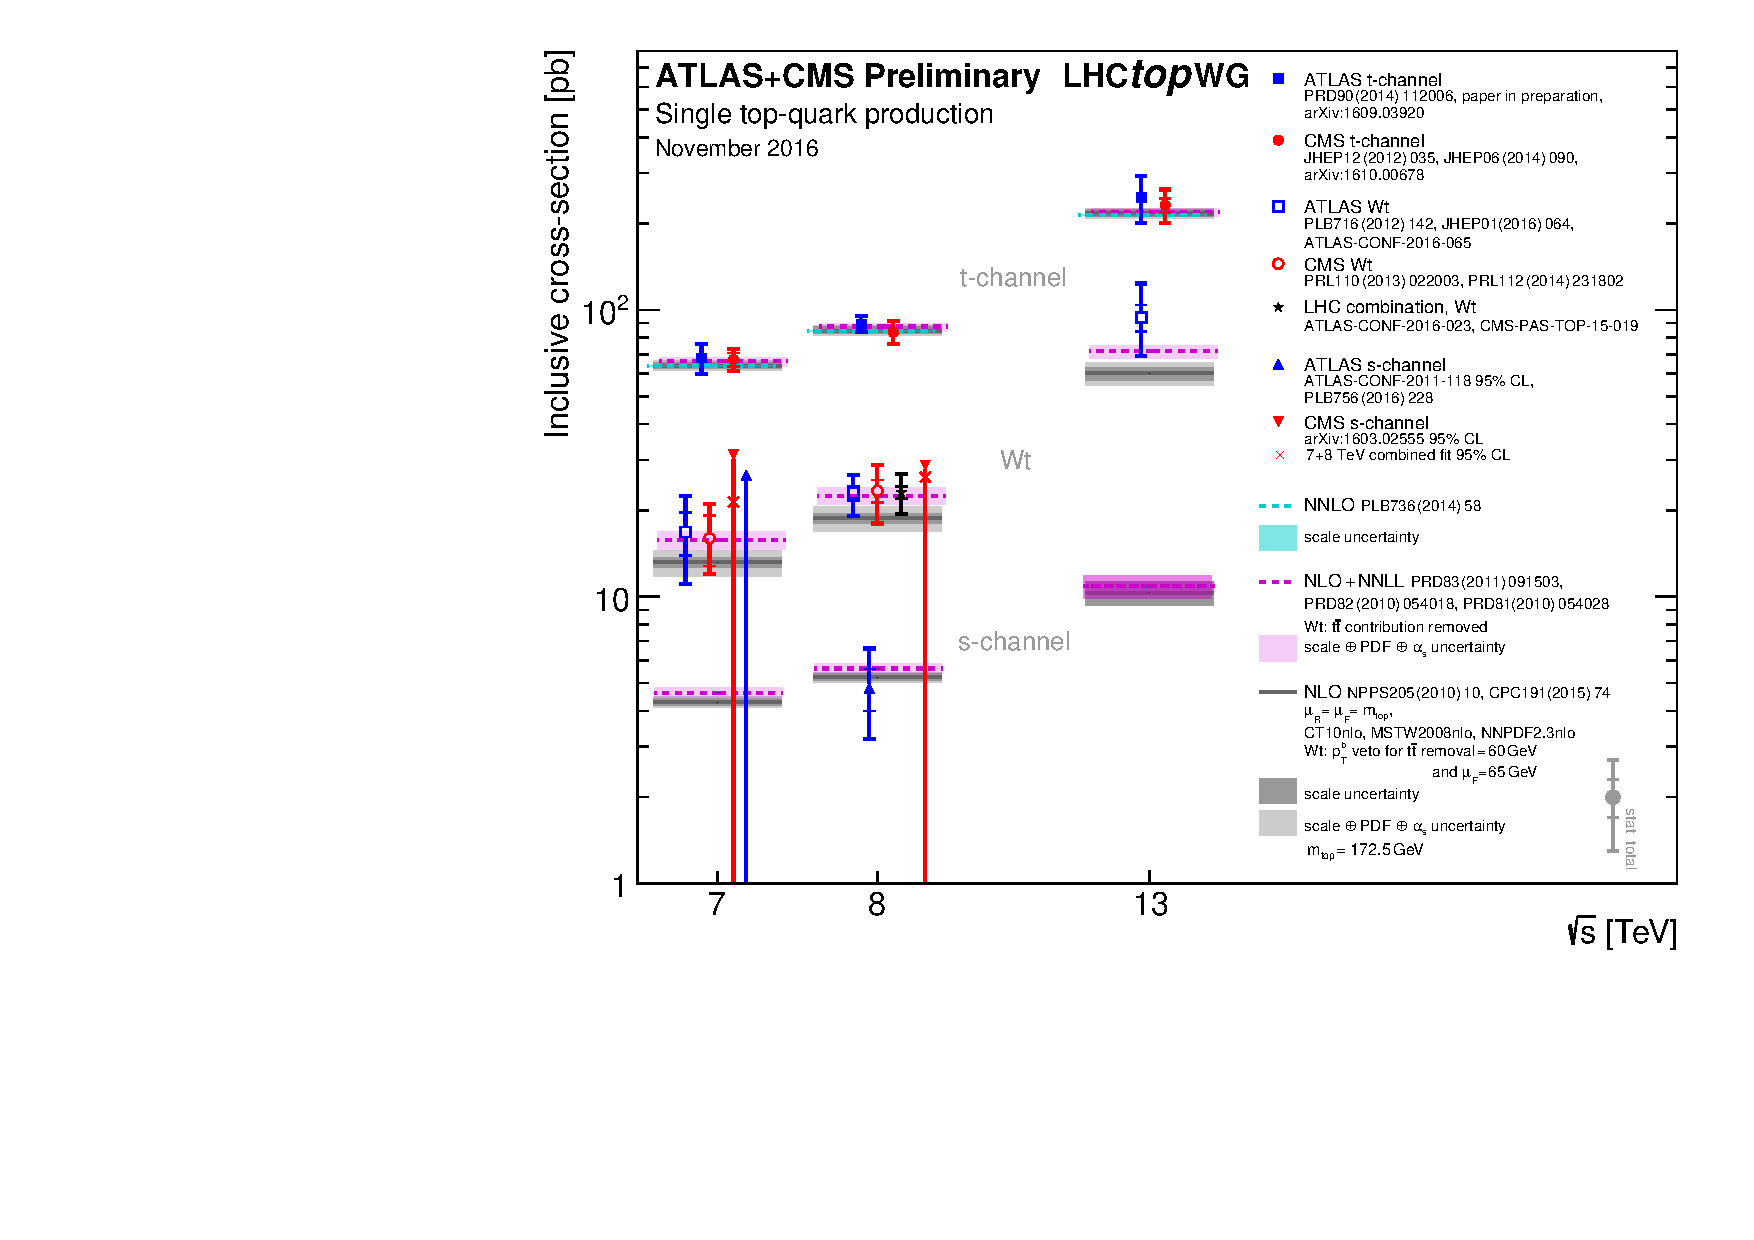
\includegraphics[width=0.9\textwidth]{figures/theory/LHC_singletop_allchannels.pdf}}
}

\myfigure[p]{\label{fig:theory-lhc-vtb}Estimations of the \gls{ckm} matrix element $\vtb$ from single-top-quark cross section measurements. The figure is taken from the TopLHC working group.}{
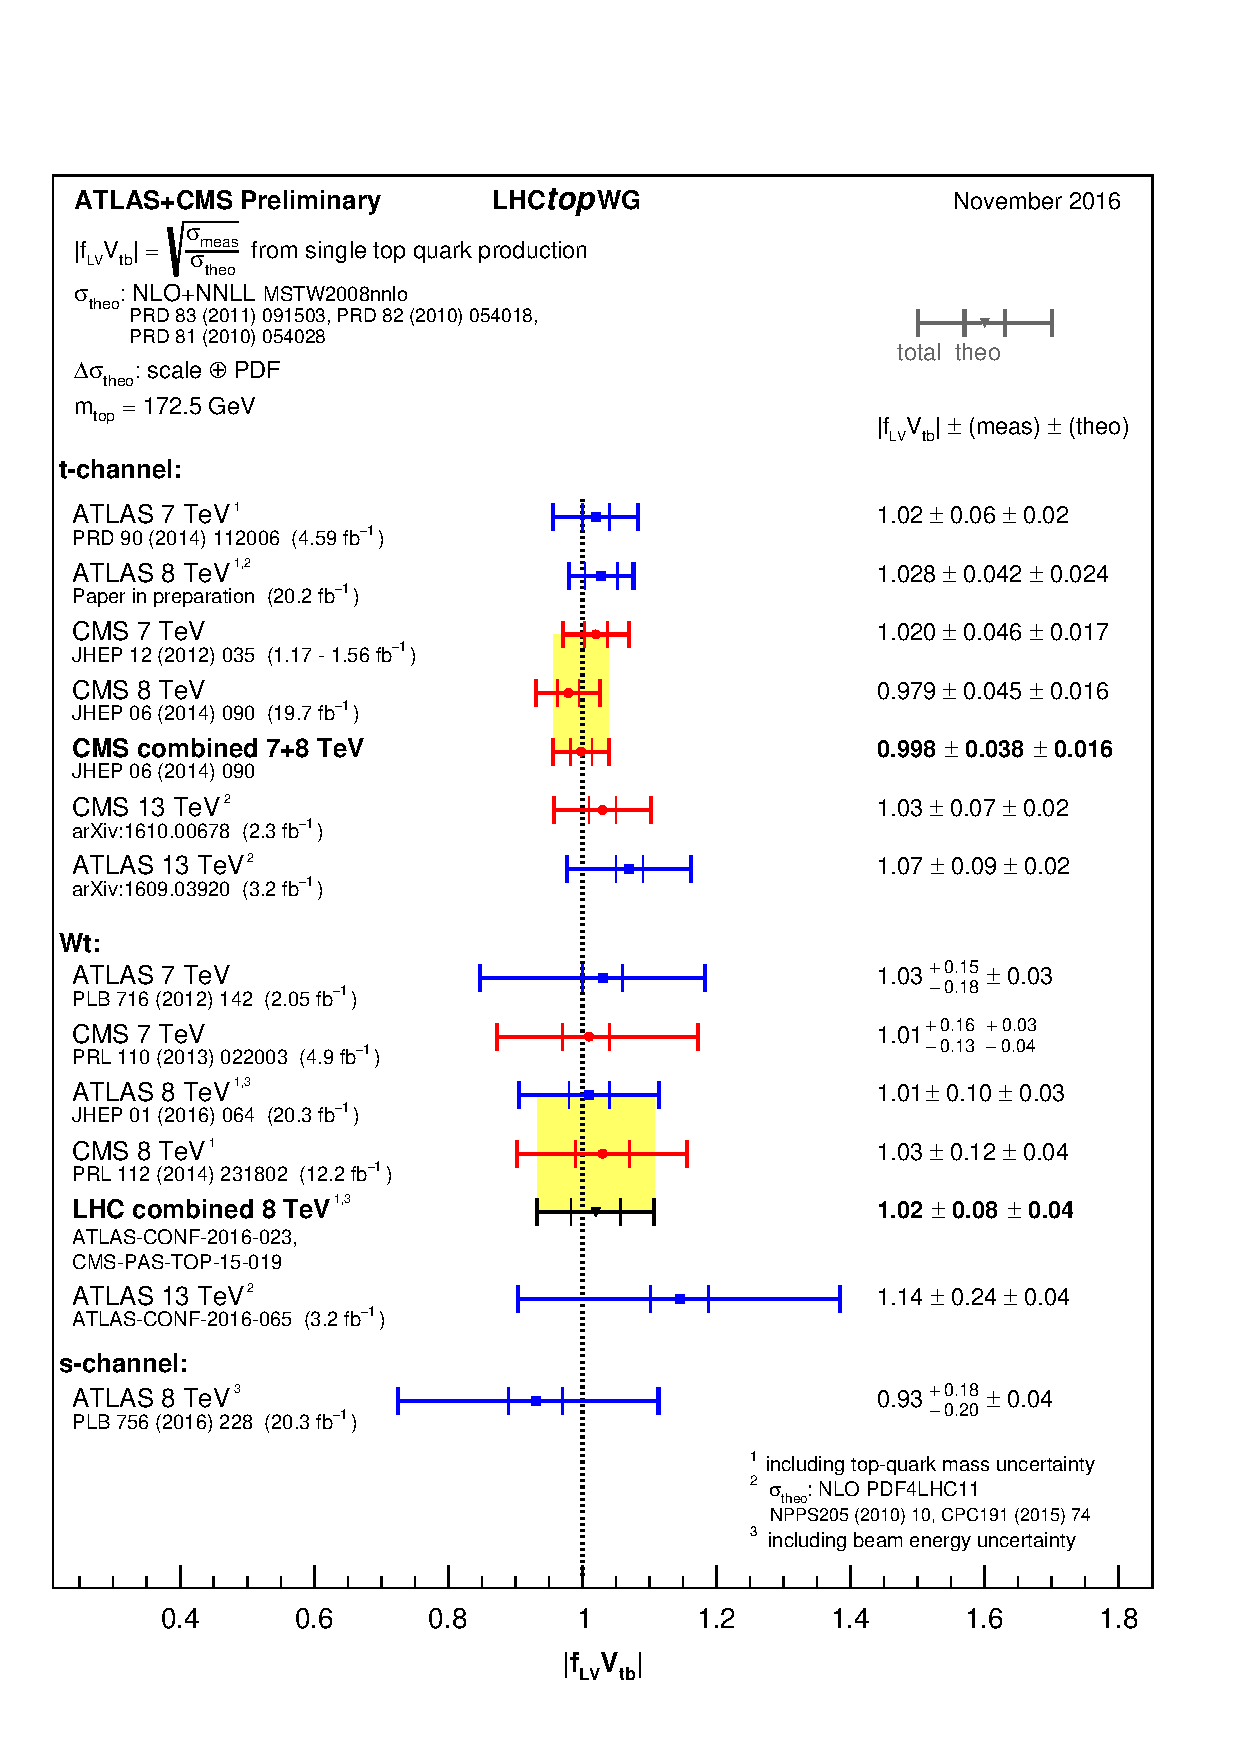
\includegraphics[width=0.99\textwidth]{figures/theory/LHC_singletop_Vtb.pdf}
}

The results from measurements of the $\mathrm{W}$~boson helicity fractions are presented in Fig.~\ref{fig:theory-lhc-whel} and compared to their \gls{nnlo} prediction. These have been mostly obtained by analyzing top quark decays in \ttbar events. However, one measurement used decays of top quarks from $t$-channel single-top-quark production yielding a comparable precision despite the lower production cross section~\cite{Khachatryan:2014vma}.

\myfigure[htbp]{\label{fig:theory-lhc-whel}Overview of $\mathrm{W}$~boson helicity fraction measurements. The figure is taken from the TopLHC working group.}{
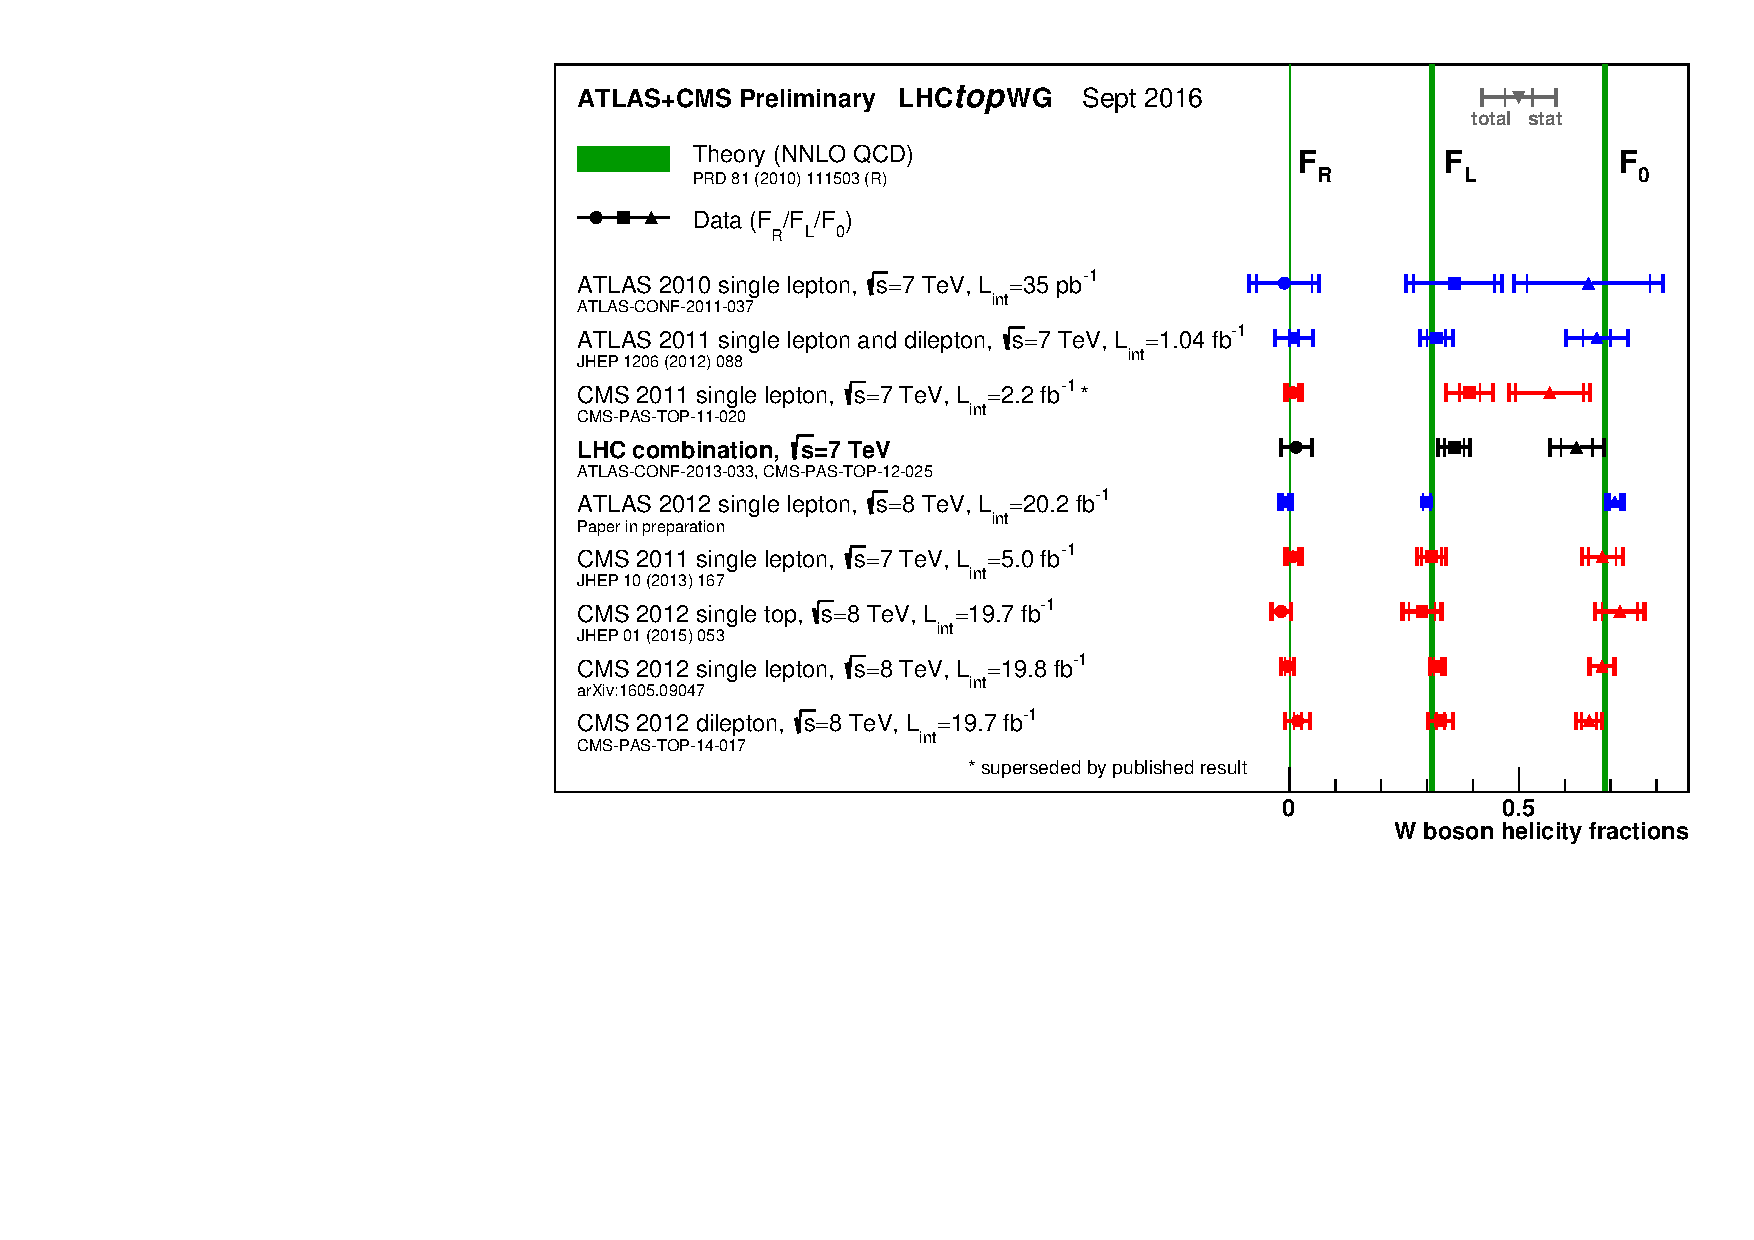
\includegraphics[width=0.95\textwidth]{figures/theory/LHC_W_helicity.pdf}
}

Overall, the various measurements presented here show a good agreement with the \gls{sm} prediction. Since no deviation is observed, limits on the anomalous couplings can be derived. Global fits of the anomalous couplings are however a complicated and computing-intense undertaking. Given a certain point in the coupling hyperspace, multiple observables need to be computed and compared to the results from various measurements. Statistical and systematic uncertainties need to be incorporated into the fitting procedure as well. A sophisticated fitting framework called \textsc{TopFitter} has been recently developed~\cite{Buckley:2015lku}. The current estimates per operator contributing to single-top-quark production obtained from various \gls{lhc} and Tevatron measurements are shown in Fig.~\ref{fig:theory-eft-fit}. The results are found to be consistent with the \gls{sm} expectation where those operators vanish.

\myfigure[htbp]{\label{fig:theory-eft-fit}Estimates per operator contributing to single-top-quark production. Shown are 95\% confidence intervals. The Wilson coefficient $C_\mathrm{t}$ contains all contributions from four-fermion interactions. The figure is taken from Ref.~\cite{Buckley:2015lku}.}{
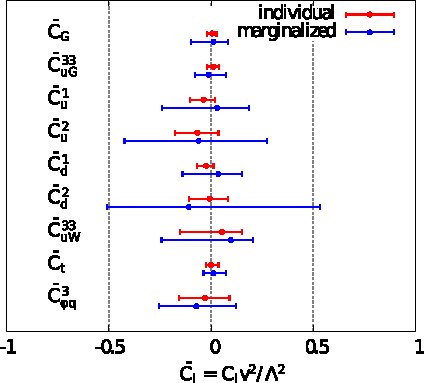
\includegraphics[scale=0.85]{figures/theory/EFT_fit.pdf}
}




